The given information is summarised in Table \ref{constr/56/tab}.
\begin{table}[!ht]
\begin{center}
    \resizebox{\columnwidth}{!}{
\begin{tabular}{ | c | c| c| c |} 
\hline
& Symbols & Circle1 & Circle2 \\
\hline
Centre & $\vec{O}$ & \myvec{0\\0} & \myvec{0\\0} \\ 
\hline
Radius & $r_{1}$,$r_{2}$ & 4 & 6\\ 
\hline
\end{tabular}
}
\end{center}
\caption{}
\label{constr/56/tab}
\end{table}
See Fig. \ref{fig:constr/56/Tangent}. Let P be a point on Circle 2 with radius 6.  Then 
\begin{align}
\vec{P} = \myvec{6\\0}
\end{align}
Let $PQ$ and $PR$  be tangents from point $\vec{P}$ on circle with radius 6 to the points $\vec{Q}$ and $\vec{R}$ on circle with radius 4 .
% \begin{align}
% \because OQ \perp QP,
% \end{align}
Now,
\begin{align}
(\vec{O}-\vec{Q})^T (\vec{Q}-\vec{P}) &= 0 \quad \brak{\because OQ \perp QP }
% \\
% \vec{Q}^T(\vec{Q}-\vec{P}) &= 0 \quad \brak{\because \vec{O}=\myvec{0\\0}}
% \\
% \vec{Q}^T \vec{Q} - \vec{Q}^T \vec{P} &= 0  
% \\
% \norm{\vec{Q}}^2 &= \vec{Q}^T \vec{P}
% \\
% \norm{\vec{Q}}^2 &= \vec{P}^T \vec{Q}  \quad \brak{\because \vec{Q}^T \vec{P} = \vec{P}^T \vec{Q}}
\\
\implies \vec{P}^T \vec{Q} &= 16 \quad \brak{\because \norm{\vec{Q}}^2 = 16}
% \\
% \myvec{6&0} \vec{Q} &= 16 \quad \brak{\because \vec{P} = \myvec{6\\0} }
\\
\text{or, }\myvec{1&0} \vec{Q} &= \frac{8}{3}
\\
\implies \vec{Q} &= \myvec{\frac{8}{3}\\0} + \lambda \myvec{0\\1} \label{constr/56/2.0.11} 
\\
&=\vec{q}+\lambda\vec{m}
\\
\text{where }\vec{q}&=\myvec{\frac{8}{3}\\ 0},\vec{m}=\myvec{0\\1}
\end{align}
We know,
\begin{align}
\norm{\vec{q}+\lambda\vec{m}}^2&=r_1^2
\\
(\vec{q}+\lambda \vec{m})^T(\vec{q}+\lambda \vec{m})&=r_1^2
\\
\lambda^2&=\frac{r_1^2-\norm{\vec{q}}^2}{\norm{\vec{m}}^2}
\\
\lambda &= \pm 2.98
\end{align}

Substituting the above in \eqref{constr/56/2.0.11},
%
\begin{align}
\vec{Q}=\myvec{\frac{8}{3}\\2.98},
\vec{R}=\myvec{\frac{8}{3}\\-2.98}
\end{align}
The circels as well as the tangents are plotted in Fig.     \ref{fig:constr/56/Tangent}
%
\begin{figure}[ht]
    \centering
    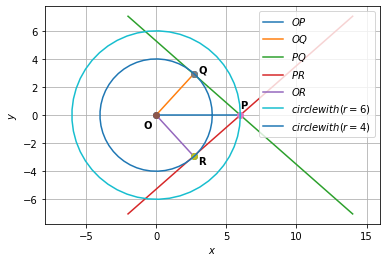
\includegraphics[width=\columnwidth]{solutions/circle/56/TANGENT.png}
    \caption{Tangent lines to circle of radius 4 units.}
    \label{fig:constr/56/Tangent}
\end{figure}    



